\chapter{Citations and Images} \label{citationsandimages}

Section \ref{citations} presents citations example. Section \ref{images} introduces an example of including
an image in a Figure context.

\section{Citations} \label{citations}

This section includes various citations examples. For example, one protagonist of the thesis this document
is based on is the MDS robot platform \cite{MDS}. The MDS has many sensors, including a Firefly Firewire
camera \cite{FireflyDatasheet}. Another feature of the MDS platform is its IRCP network communication
protocol \cite{IRCP}.

The Camshift (Continuously Adaptive Mean Shift) algorithm
is described in the article \cite{BradskiCamshift}. Finally, citations can also be included in foot notes. 
\footnote{OpenCV \cite{Bradski} implements the extended version of the Viola-Jones detector described by
Lienhart and Maydt \cite{Lienhart}.}

\section{Images} \label{images}

Figure \ref{imageexample} shows a sample image.

\begin{figure}[t]
\center
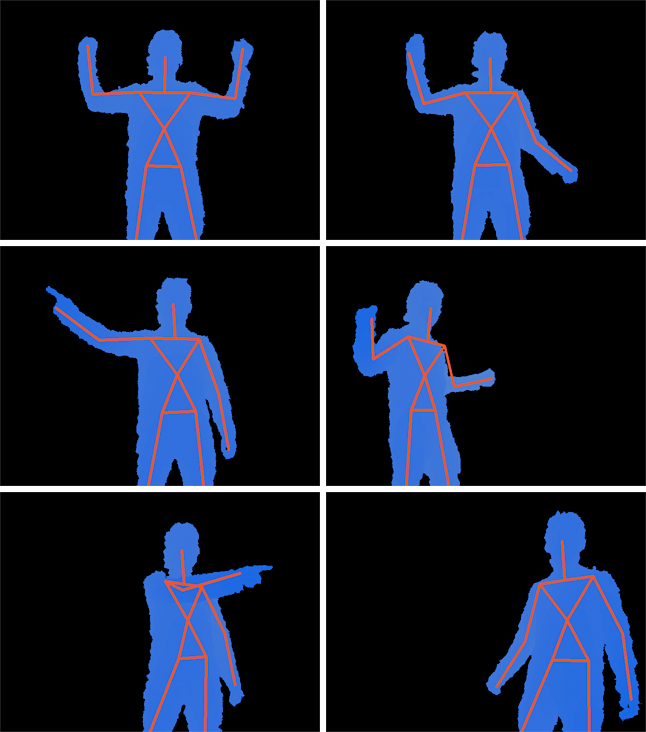
\includegraphics[width = 10cm]{sample.png}
\caption[Example of a figure with an image]{Example of including an image inside a \texttt{figure} using command \texttt{includegraphics}.}
\label{imageexample}
\end{figure}